\section{Style sheet}


\begin{frame}
     \begin{enumerate} \setlength{\itemsep}{2mm}
	\item Разделять пустыми строками всё, что только можно: слайды, теоремы внутри слайдов. Только {\tt center} и {\tt equation*} начинаются на той же строке, что и код до них.

	\item Что-то пошло не так, и для теорем на русском пришлось использовать другие окружения. Зато их названия короче оригинальных.

	\item Каждый topic, который мы оформляем индивидуально,~— это {\tt section} и отдельный файл. Презентации по дням~— или одну общую~— потом как-то из них склеим.

	\item Картинки {\it не} складируются в корневой папке.

	\item Цвета можно брать \underline{\href{https://www.latextemplates.com/images/svgnames.jpg}{отсюда.}} И ещё несколько определены в стилевике.
     \end{enumerate}
\end{frame}


\section{Minimal working example}


\begin{frame}{Слайд}
	Sample text

\begin{block}{Block title}
	Блок с заголовком
\end{block}

\vspace{-1.4ex} \begin{block}{\vspace*{-3ex}}
	Блок без заголовка
\end{block}
\end{frame}


\subsection{Technical assets}


\begin{frame}{Теоремы}
\begin{thm}[Безымянного]
	То, что да, оно да.
\end{thm}

\begin{lm}
	То, что нет, оно нет.
\end{lm}

\begin{task}
	Доказать, что то, что ну типа, оно ну типа.
\end{task}
\end{frame}


\begin{frame}{Тикз}
	\begin{center} 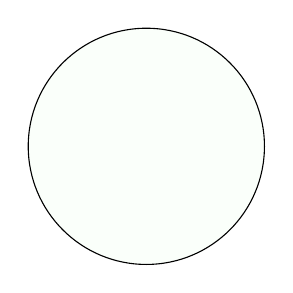
\begin{tikzpicture}
	     \filldraw[fill=Honeydew,fill opacity=0.3] (0,0) circle[radius=1.5cm];
	\end{tikzpicture}\end{center}
\end{frame}
